\begin{figure}[ht]
\centering
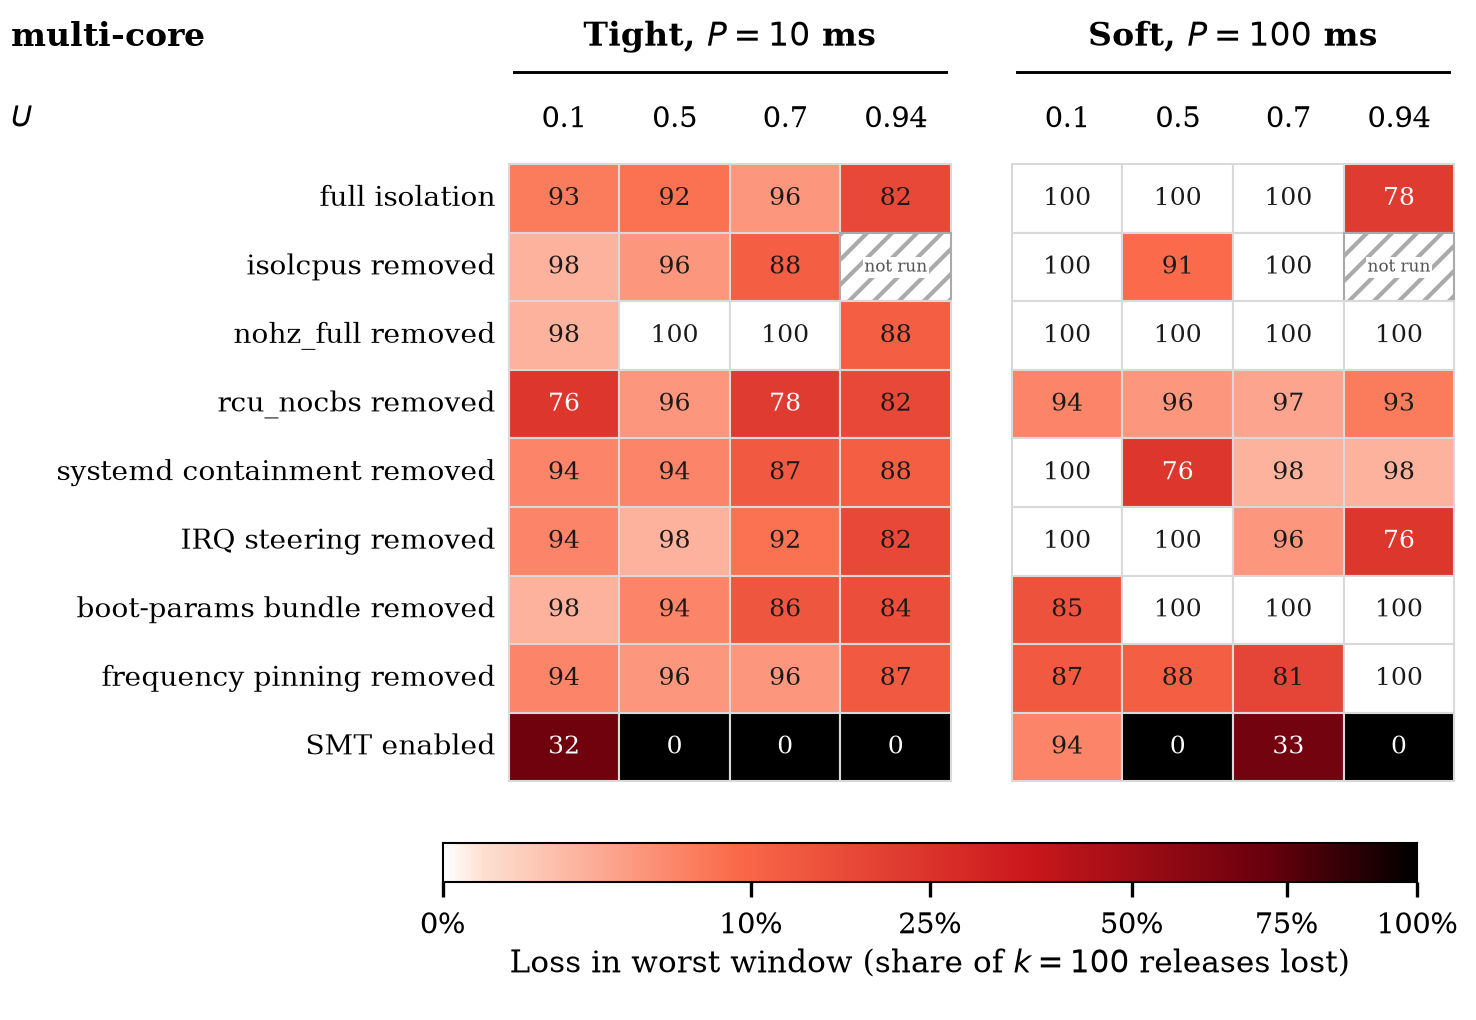
\includegraphics[width=\textwidth]{heatmap_multi-core.png}
\caption{Worst window of $k = 100$ consecutive releases for every configuration, period and utilization, multi-core. Each cell gives $m$, the smallest number of releases that met their deadline and were not skipped in any window of 100 releases. Cells with $m = 100$ have no colour; the more releases lost, the more intense the red, and black means that every release of the window was lost. The colour follows the loss $(k-m)/k$ on a \emph{square-root} scale, so that small losses stay distinguishable from zero. The first six jobs after every restart are excluded. Hatched cells were not run.}
\label{fig:rq1-heatmap-multi-core}
\end{figure}
